\documentclass{article}
\usepackage[a4paper, margin=1in]{geometry}
 \usepackage{graphicx}

\title{Informação Profissional em Ciência da Computação:\\
	Seminário Arquitetura de Computadores}
\author{
    Carlos Eduardo Gallo Filho \\
	Caio Uehara Martins \\
	Pedro}
\date{\today}

\begin{document}
\maketitle
\graphicspath{ {./images/} }

\section{Introdução}
\subsection{Arquitetura x Organização}
\subsection{Estrutura x função}
\subsection{Estrutura single core x multi core}
\subsection{Estrutura interna do core}

\section{Breve história dos computadores: Primeira geração}
\begin{flushleft}
    \qquad A primeira geração de computadores é conhecida pelo uso das válvulas para representar os elementos lógicos digitais e a memória. E também, o  \textit{conceito de programa armazenado}, atribuída ao matemático John Von Neumann, que surgiu para a construção do computador EDVAC (Eletronic Discrete Variable Computer), mas foi principalmente discutido no desenvolvimento do computador IAS, o qual é um protótipo para quase todos os computadores de propósito geral de hoje em dia. 
\end{flushleft}

\subsection{Arquitetura de Von Neumann}
\begin{center}
    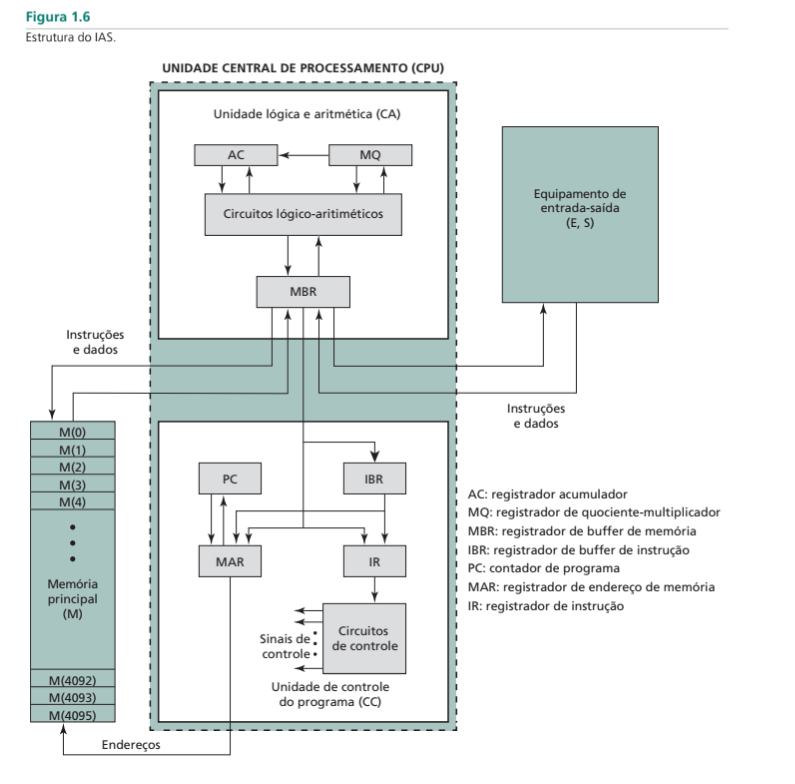
\includegraphics[scale=1]{estruturaDoIAS.jpg}
    \qquad
\end{center}


\subsection{Descrição dos elementos de Von Neumann}
\subsection{Endereçamento de memória}

\section{Breve história dos computadores: Segunda geração}
\section{Breve história dos computadores: Terceira geração}
\section{Breve história dos computadores: Gerações posteriores}

\end{document}